\begin{frame}
    \usebeamerfont{title}\usebeamercolor[fg]{title}Tests\par
\end{frame}

\begin{frame}{Set up}
8 Agents with 4 CPU(s), 8-16 GB of RAM, and 45 GB of Disk.

\begin{center}
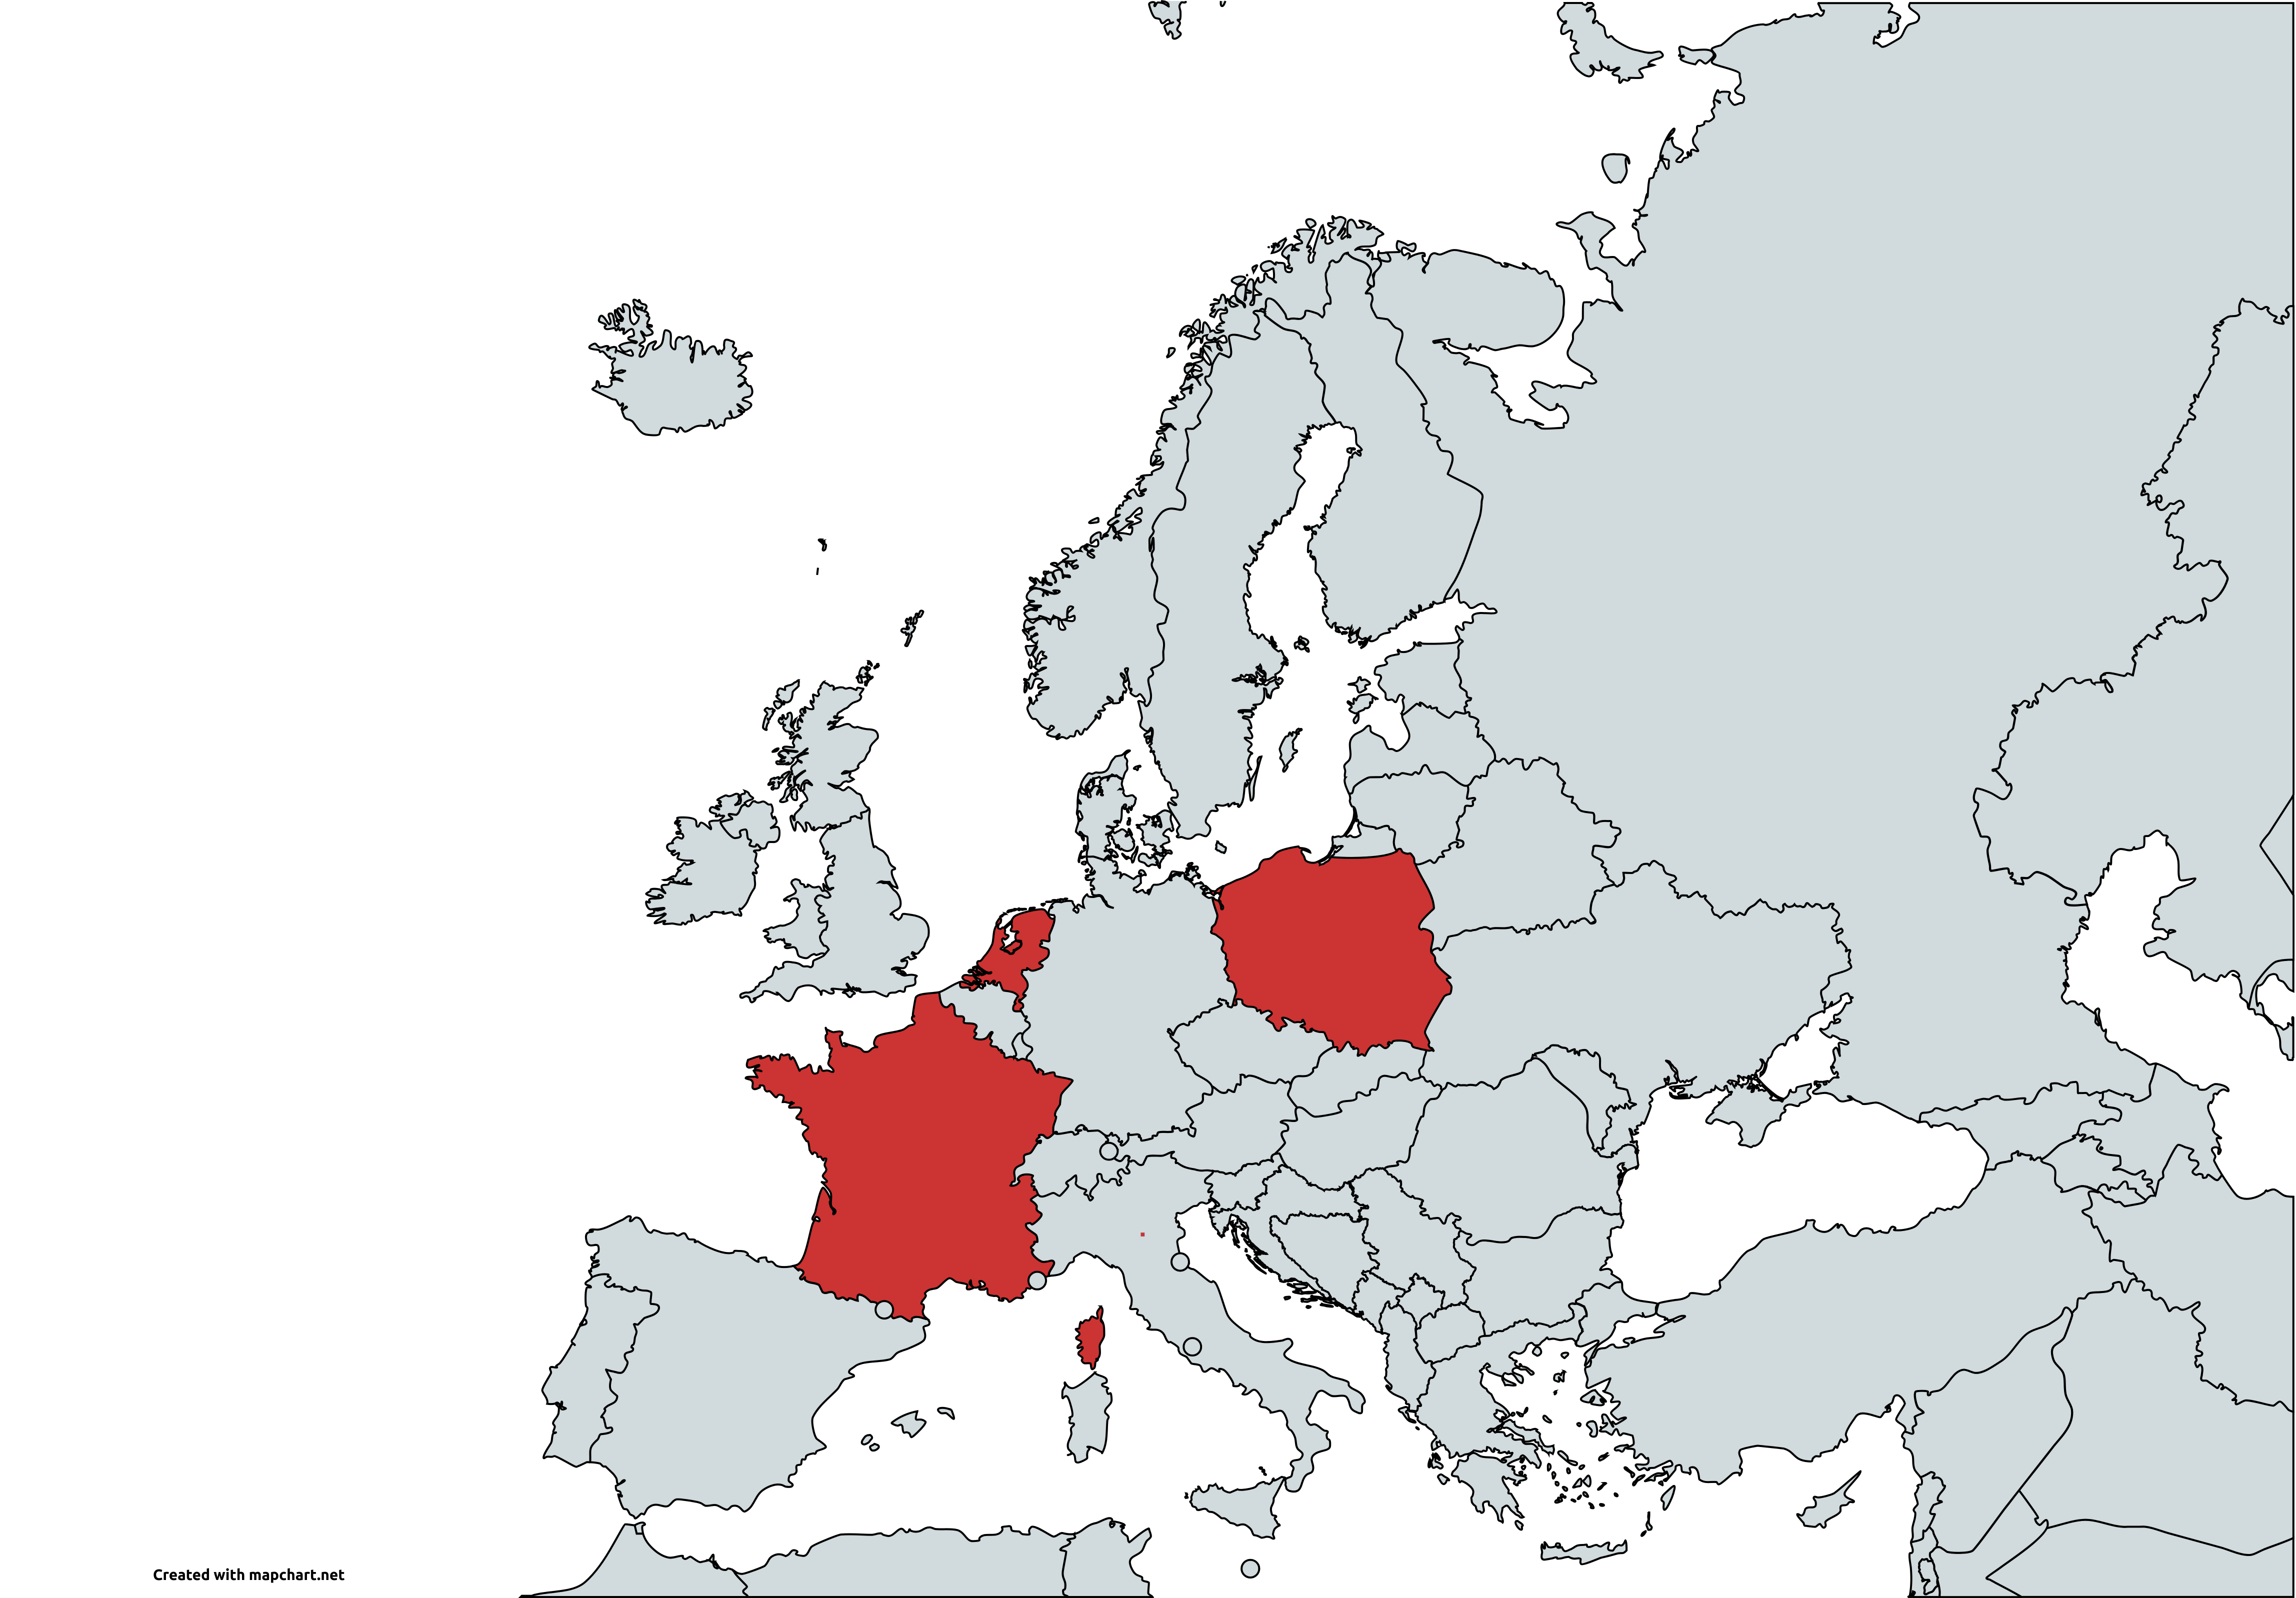
\includegraphics[width=0.5\linewidth]{static/map-chart.png}
\end{center}

\only<2>{Per each test let's consider: number of online/offline Agents and file
sizes and counts.}

\end{frame}

\begin{frame}{Same dataset but different file size and count -- 1}

\begin{figure}
\centering
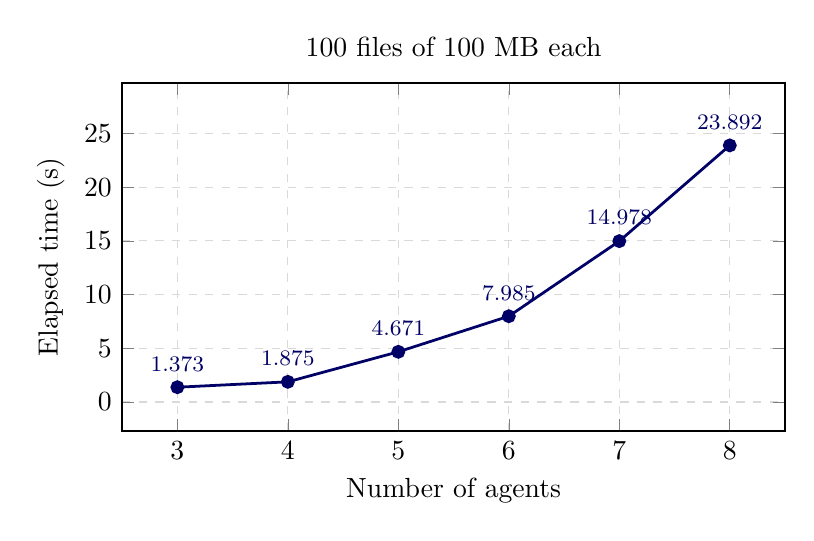
\begin{tikzpicture}
\begin{axis}[
    width=10cm, height=6cm,
    xlabel={Number of agents},
    ylabel={Elapsed time (s)},
    xmin=3, xmax=8,
    ymin=0, ymax=27,
    xtick={3,4,5,6,7,8},
    ytick={0,5,10,15,20,25},
    grid=major,
    grid style={dashed,gray!30},
    thick,
    title={100 files of 100 MB each},
    enlargelimits=0.1,
    clip=false,
    nodes near coords,
    every node near coord/.append style={font=\footnotesize, anchor=south, yshift=2pt},
    point meta=explicit symbolic
]

\addplot[color=blue!40!black, mark=*, line width=1pt] coordinates {
    (3,1.373) [1.373]
    (4,1.875) [1.875]
    (5,4.671) [4.671]
    (6,7.985) [7.985]
    (7,14.978) [14.978]
    (8,23.892) [23.892]
};
\end{axis}
\end{tikzpicture}
\end{figure}

\end{frame}

\begin{frame}{Same dataset but different file size and count -- 2}

\begin{figure}
\centering
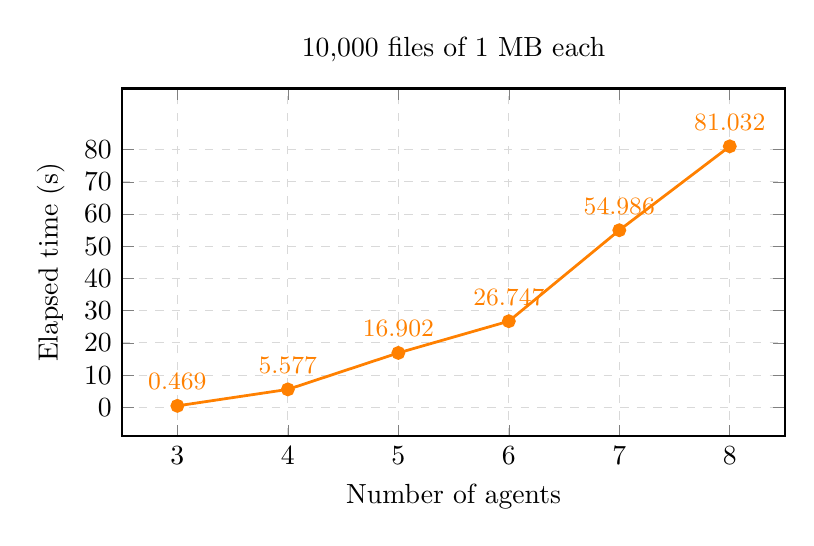
\begin{tikzpicture}
\begin{axis}[
    width=10cm, height=6cm,
    xlabel={Number of agents},
    ylabel={Elapsed time (s)},
    xmin=3, xmax=8,
    ymin=0, ymax=90,
    xtick={3,4,5,6,7,8},
    ytick={0,10,20,30,40,50,60,70,80},
    grid=major,
    grid style={dashed,gray!30},
    thick,
    title={10,000 files of 1 MB each},
    enlargelimits=0.1,
    clip=false,
    nodes near coords,
    every node near coord/.append style={font=\small, anchor=south, yshift=2pt},
    point meta=explicit symbolic
]

\addplot[color=orange, mark=*, line width=1pt] coordinates {
    (3,0.4685) [0.469]
    (4,5.577) [5.577]
    (5,16.902) [16.902]
    (6,26.747) [26.747]
    (7,54.986) [54.986]
    (8,81.032) [81.032]
};
\end{axis}
\end{tikzpicture}
\end{figure}

\end{frame}

\begin{frame}{Same dataset but different file size and count -- 3}

\begin{figure}
\centering
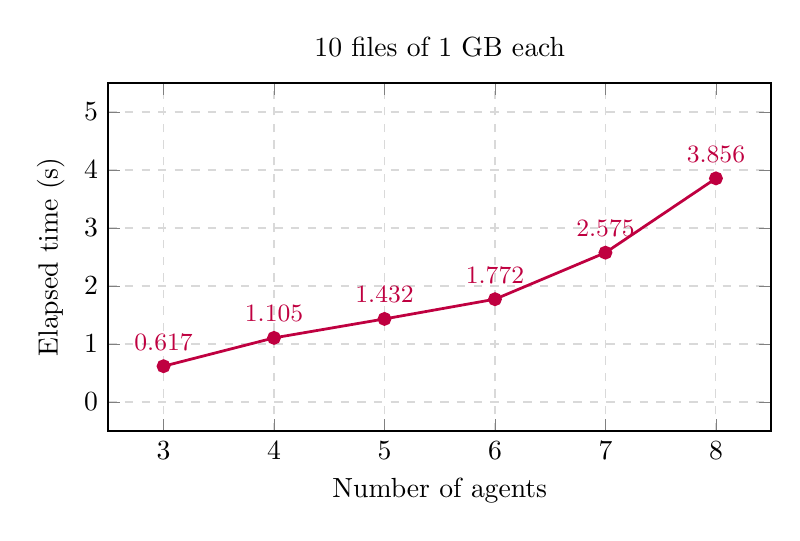
\begin{tikzpicture}
\begin{axis}[
    width=10cm, height=6cm,
    xlabel={Number of agents},
    ylabel={Elapsed time (s)},
    xmin=3, xmax=8,
    ymin=0, ymax=5,
    xtick={3,4,5,6,7,8},
    ytick={0,1,2,3,4,5},
    grid=major,
    grid style={dashed,gray!30},
    thick,
    title={10 files of 1 GB each},
    enlargelimits=0.1,
    clip=false,
    nodes near coords,
    every node near coord/.append style={font=\small, anchor=south, yshift=2pt},
    point meta=explicit symbolic
]

\addplot[color=purple, mark=*, line width=1pt] coordinates {
    (3,0.6166) [0.617]
    (4,1.105) [1.105]
    (5,1.432) [1.432]
    (6,1.772) [1.772]
    (7,2.575) [2.575]
    (8,3.856) [3.856]
};
\end{axis}
\end{tikzpicture}
\end{figure}

\end{frame}

\begin{frame}{Test with offline agents}

\begin{figure}
\centering
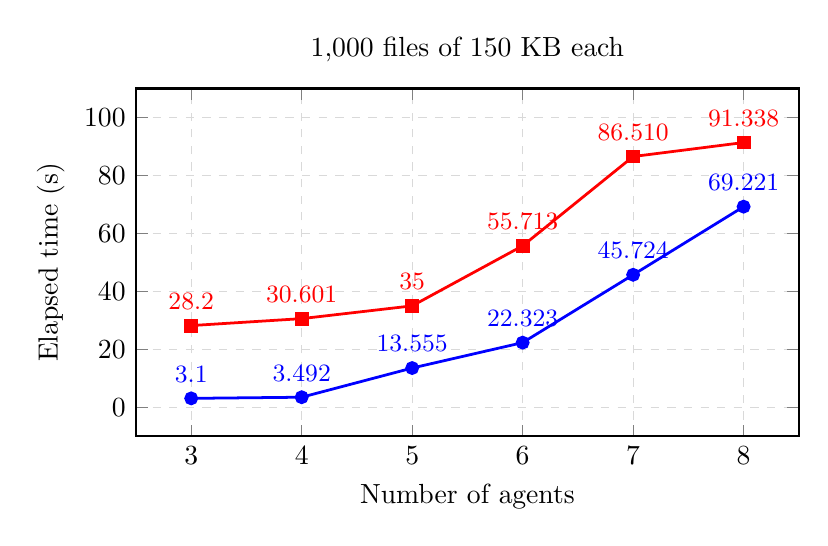
\begin{tikzpicture}
\begin{axis}[
    width=10cm, height=6cm,
    xlabel={Number of agents},
    ylabel={Elapsed time (s)},
    xmin=3, xmax=8,
    ymin=0, ymax=100,
    xtick={3,4,5,6,7,8},
    ytick={0,20,40,60,80,100},
    grid=major,
    grid style={dashed,gray!30},
    thick,
    title={1,000 files of 150 KB each},
    enlargelimits=0.1,
    clip=false,
    nodes near coords,
    every node near coord/.append style={font=\small, anchor=south, yshift=2pt},
    point meta=explicit symbolic
]

% Online agents
\addplot[color=blue, mark=*, line width=1pt] coordinates {
    (3,3.1) [3.1]
    (4,3.492) [3.492]
    (5,13.555) [13.555]
    (6,22.323) [22.323]
    (7,45.724) [45.724]
    (8,69.221) [69.221]
};

% Offline agents
\addplot[color=red, mark=square*, line width=1pt] coordinates {
    (3,28.2) [28.2]
    (4,30.601) [30.601]
    (5,35) [35]
    (6,55.713) [55.713]
    (7,86.510) [86.510]
    (8,91.338) [91.338]
};

\end{axis}
\end{tikzpicture}
\end{figure}

\end{frame}

\begin{frame}{Test with very large number of tiny files}

\begin{figure}
\centering
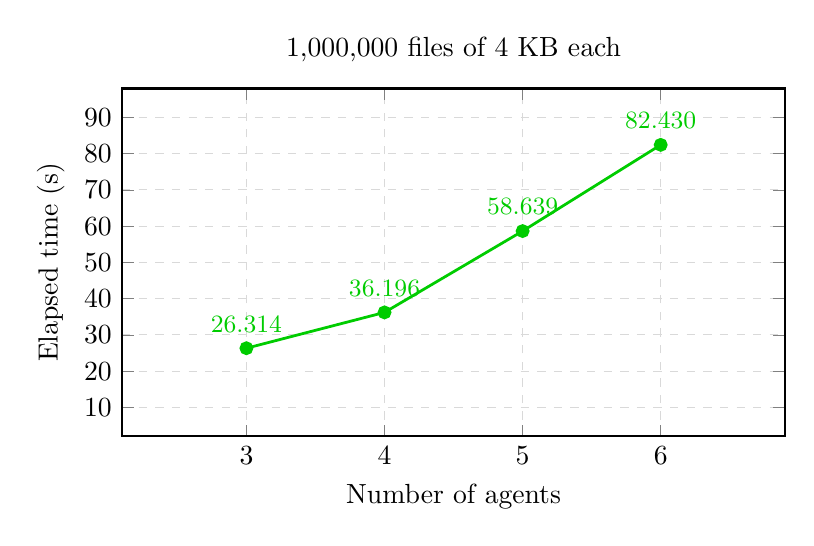
\begin{tikzpicture}
\begin{axis}[
    width=10cm, height=6cm,
    xlabel={Number of agents},
    ylabel={Elapsed time (s)},
    xmin=2.5, xmax=6.5,
    ymin=10, ymax=90,
    xtick={3,4,5,6},
    ytick={0,10,20,30,40,50,60,70,80,90,100},
    grid=major,
    grid style={dashed,gray!30},
    thick,
    title={1,000,000 files of 4 KB each},
    enlargelimits=0.1,
    clip=false,
    nodes near coords,
    every node near coord/.append style={font=\small, anchor=south, yshift=2pt},
    point meta=explicit symbolic
]

\addplot[color=green!80!black, mark=*, line width=1pt] coordinates {
    (3,26.314) [26.314]
    (4,36.196) [36.196]
    (5,58.639) [58.639]
    (6,82.430) [82.430]
};
\end{axis}
\end{tikzpicture}
\end{figure}

\end{frame}

\begin{frame}{Results}
\begin{itemize}
\item Scenarios with many small files amplify the cost of synchronization and
consensus.
\item Verification time increases with the number of agents and files.
\item Confirmed the correctness and resilience of the approach under different scenarios and network conditions.
\end{itemize}
\end{frame}

\begin{frame}{Conclusion}
\begin{itemize}
\item Raft ensures that integrity metadata is synchronized cluster-wide, while Merkle trees allow hierarchical and efficient integrity checks at the folder or subfolder level.
\item<2> It is possible to maintain a consistent and verifiable integrity state across distributed agents without relying on full file scans or constant node availability.
\end{itemize}
\end{frame}


\begin{frame}
\centering
    \usebeamerfont{title}\usebeamercolor[fg]{title}Thank you for the attention.\par
\end{frame}
